\chapter{Minimal Manhattan network (MMN)}
At this stage, most of the work is already done, we just only miss the computation of the minimal Manhattan network.

Clearly, with all the data we have now from our set it will be (with the usage of some tricks) easy to compute it.

Now that we have the Pareto envelope of our set, we just need to find a generating set over our terminals and satisfy it.

In this chapter we will cover what is a generating set and why satisfying such a set is equivalent to finding a minimal Manhattan network.
\section{Generating set}%%%%%%%%%%%%%%%%%%%%%%%%%%%%%%%%%%%%%%%%
\noindent Let A be a generating set over a cloud of terminals T.

\noindent A respects the following assertions:
\begin{enumerate}[noitemsep, nolistsep]
	\item{A is a subset of T: $A \subseteq T$ }
	\item{Connecting all pairs of A \textbf{implies} All pairs of T are connected }
\end{enumerate}

\noindent As a matter of fact, we now know that we can in order to find a minimal Manhattan network, try to find a generating set over our terminals.

By studying two specific geometrical shapes in our set T we will be able to create such a generating set, thus solving our problem: finding a minimal Manhattan network.
\section{Terminal's neighbours}%%%%%%%%%%%%%%%%%%%%%%%%%%%%%%%%%
As we are trying to find geometric shapes that can be defined as a generating set, we need to be able to talk about the neighbours of a point.

In fact we will create appropriated data structures so that we keep in memory the neighbours of each point.

\subsection{$Q_i$, $A_i$, and $O_i$ dictionaries.}
\noindent For that we will use dictionaries:
\begin{itemize}[noitemsep, nolistsep]
	\item{Step one: As you can see in \emph{Fig 8.1} is for a point to divide the space around it in four squares. ($Q_i$ $|$ $\forall i \in [1,4]$) }
	\item{Step two: For each $Q_i$ we will create the appropriated $A_i$ and $O_i$}
\end{itemize}

\begin{figure}[H]
  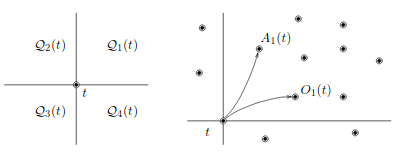
\includegraphics[width=\linewidth]{img/terminal_neighbours.png}
  \caption{Terminal's neighbours}
  \label{fig:terminal_neighbours}
\end{figure}

\subsection{Definition of $A_i$ and $O_i$}
\noindent Let \emph{p} and \emph{q} be two point in T. ($p \in T$ and $q \in T$)

\noindent Let $A_i$ be linked to $Q_i$. (i.e $A_1$ is linked to $Q_1$ for example)

\noindent Let $A_i$ be a dictionary from a point to another (i.e $A_i(point1) = point2$)\newline

\noindent $A_i(p) = q$ means that:
\begin{itemize}[noitemsep, nolistsep]
	\item{ $q \in Q_i$}
	\item{ \emph{q} is the closest point to the a \textbf{vertical line} going through \emph{p}}
\end{itemize}

\noindent $O_i(p) = q$ means that:
\begin{itemize}[noitemsep, nolistsep]
	\item{ $q \in Q_i$}
	\item{ \emph{q} is the closest point to the an \textbf{horizontal line} going through \emph{p}}
\end{itemize}

\subsection{Algorithm to create $A_i$ and $O_i$}
In this part I will present you an algorithm to generate $O_1$.

\noindent \textbf{Note:} All other dictionaries can be created similarly just by giving small modifications on the following algorithm.
 
\begin{algorithm}[H]
\SetAlgoLined
 \caption{Calculate $O_1$}
\KwResult{The $0_1$ dictionary properly filled }
Sort T  by increasing ordinates and increasing abscissa\;
$O_1 = $ An empty dictionary\;
toTreat = An empty stack\;
$toTreat.push( t_0)$\;
\For{ i=1 to n }{
	\While{ First element of toTreat has an abscissa $\leq x_{t_i}$ }{
		s = toTreat.pop()\;
		$O_1(s) = t_i$\;
	}
	toTreat.push($t_i$)\;
}
\While{The stack toTreat is not empty}{
	s = toTreat.pop()\;
	$O_1(s) = \o$\;
}
return $O_1$
\end{algorithm}


\section{Strips}%%%%%%%%%%%%%%%%%%%%%%%%%%%%%%%%%%%%%%%%%%%%%%%%
In this section we will cover strips which are composed with the set of vertical and horizontal strips created by our points.
\subsection{What are strips}
Vertical(reps. Horizontal) strips are geometrical forms made by two points that are successive in y(reps. x) coordinate.
\begin{figure}[H]
  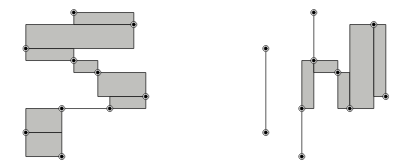
\includegraphics[width=\linewidth]{img/strips.png}
  \caption{Vertical and horizontal strips.}
  \label{fig:strips}
\end{figure}
\subsection{Algorithm to locate strips}
\begin{algorithm}[H]
\SetAlgoLined
 \caption{LocateStrip}
\KwResult{HS and VS as lists of tuples. (respectively horizontal strips and vertical strips}
 HS = \o\;
 VS = \o\;
 Calculate $O_i$ and $A_i$ $|$ $ \forall i \in [1,4]$\;
 \For{i=1 to n}{
 	\uIf{$t_i = O_3(O_1(t_i))$}{
 		$HS = HS\cup (t_i,O_1(t_i))$\;
	}
 	\uIf{$t_i = O_4(O_2(t_i))$}{
 		$HS = HS\cup (t_i,O_2(t_i))$\;
 	}
 	\uIf{$t_i = A_3(A_1(t_i))$}{
 		$VS = VS\cup (t_i,A_1(t_i))$\;
 	}
 	\uIf{$t_i = A_4(A_2(t_i))$}{
 		$VS = VS\cup (t_i,A_2(t_i))$\;
 	}
 }
 return HS and VS\;
\end{algorithm}

\section{Staircases}%%%%%%%%%%%%%%%%%%%%%%%%%%%%%%%%%%%%%%%%%%%%
Staircases are another geometric shape with a specific configuration.
\begin{figure}[H]
  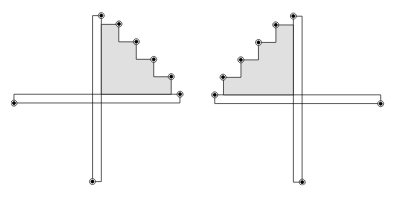
\includegraphics[width=\linewidth]{img/staircases.png}
  \caption{Staircases configuration.}
  \label{fig:staircases} 
\end{figure}

Here above on \emph{Fig 8.3} are presented two of the four possible staircases configuration.

As you can see a staircase is built on two strips, one vertical and the other one horizontal. Also note the position of the points on the strips. The points must be on a disposition where the points on the staircase side are part of the staircase itself.
\section{The resulting set}%%%%%%%%%%%%%%%%%%%%%%%%%%%%%%%%%%%
Now that we have strips and staircases we can create a generating set.

In fact all strips combined with all staircases are a generating set for our cloud of points.

Meaning that at this point we can now with the data that we have, instead of treating all terminals we can just focus on our staircases and strips.
